\section{Raccolta dati}

I dati riguardanti la simulazione sono stati raccolti a partire dall'1 marzo 2020 fino al 27 giugno 2020 per un arco di tempo di circa 4 mesi, al ritmo di 1,200 richieste al giorno. L'Italia è entrata in uno stato di lockdown nazionale per emergenza COVID19 il 12 marzo e ha allentato le restrizioni a partire dal 4 maggio. I dati raccolti a partire da quest'ultima data sono considerati validi per le analisi. Sono stati salvati in formato .csv, dove ogni riga contiene le seguenti informazioni:

\begin{center}
	\begin{tabular}{ | c | c | c | c | c | c | c | c | c | }
		\hline
		Data & Orario & Partenza & Arrivo & Auto & ATM & Enjoy & Bici & Piedi \\
		\hline
	\end{tabular}
\end{center}

In partenza e arrivo sono salvate le coordinate espresse in gradi del tragitto generato, nei restanti campi le stime di percorrenza di tale tragitto espresse in minuti, insieme alla data e all'orario in cui è stata effettuata la richiesta di tale tratta.

Oltre ai dati principali sono stati salvati informazioni secondarie come il numero di auto libere Enjoy al momento della richiesta, la lunghezza aerea della tratta e la lunghezza calcolata a piedi della stessa, entrambe espresse in km.

\section{Filtro dati errati}

\begin{table}[H]
	\centering
	\begin{tabular}{ | l r r | }
		\hline
		& \textbf{n\textdegree tratte} & \textbf{\%} \\ 
		\textbf{Coerenti} & 49560 & 73 \\  
		\textbf{Errati} & 18290 & 27 \\
		\hline
		\textbf{Totale} & 67850 & 100 \\
		\hline
	\end{tabular}
	\caption{I dati errati contengono uno o più zeri nelle stime}
	\label{table:1}
\end{table}

I provider per le stime di percorrenza dei vari mezzi hanno talvolta restituto il valore zero. Questo fenomeno è probabilmente dovuto alla generazione a random delle coordinate di partenza e arrivo, che ha permesso richieste in qualsiasi punto della mappa, compresi punti non situati direttamente sulla strada come in giardini pubblici, condimini e altre zone private, o semplicemente per disservizi. Per un confronto alla pari sono state considerate solo le righe prive di zeri nel file CSV. Dalla tabella \ref{table:1}  risulta che su circa 68000 richieste, 50000 sono prive di zeri, circa il 73\% del totale.

\section{Distribuzione lunghezza tratte generate}

\begin{center}
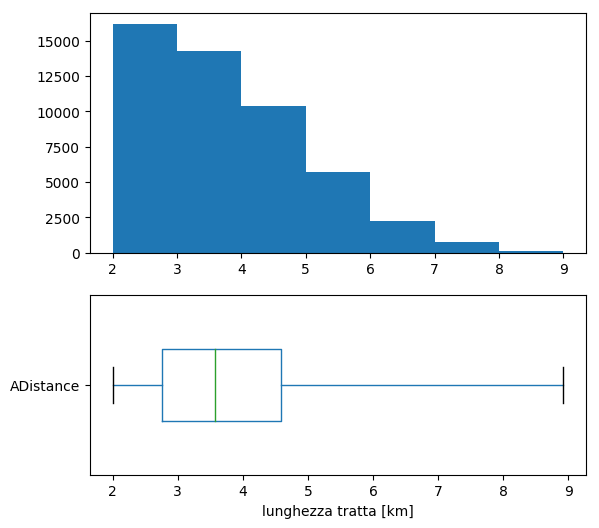
\includegraphics[scale=0.8]{distribuzione_tratte}
\end{center}

\begin{table}[H]
	\centering
	\begin{tabular}{ | l r | }
		\hline
		\textbf{Abs. freq.} & 49560 \\
		\textbf{media} & 3.80 \\
		\textbf{mediana} & 3.57 \\
		\textbf{std} & 1.27 \\
		\textbf{min} & 2.00 \\
		\textbf{max} & 9.52 \\
		\hline
	\end{tabular}
	\caption{Statistiche lunghezza tratta [km]}
	\label{table:2}
\end{table}

Nella tabella \ref{table:2} sono riportate le statistiche riguardo la lunghezza in via aerea delle tratte generate. Si può vedere come più della metà sia lunga meno di 5 km in linea aerea, risultato ottenuto in parte dai constraint imposti nella generazione.

\section{Performance medie}

\begin{table}[H]
	\centering
	\begin{tabular}{ | l r r r r r | }
		\hline
		& \textbf{Auto} & \textbf{Enjoy} & \textbf{ATM} & \textbf{Bici} & \textbf{Piedi} \\
		\textbf{media}   & 19.6 & 13.5 &  8.3 & 11.9 & 4.5 \\
		\textbf{mediana} & 19.5 & 13.2 &  7.9 & 12.0 & 4.5 \\
		\textbf{std}     &  3.9 &  3.8 &  2.3 &  1.3 & 0.0 \\
		\textbf{min}     &  6.7 &  3.0 &  3.4 &  6.5 & 4.3 \\
		\textbf{max}     & 48.5 & 36.1 & 27.8 & 16.9 & 4.6 \\
		\hline
	\end{tabular}
	\caption{Statistiche velocità media [km/h]}
	\label{table:3}
\end{table}

\section{Analisi dei singoli mezzi}

\subsection{Auto}

\subsubsection{Velocità media di ora in ora}

\begin{figure}[!h]
	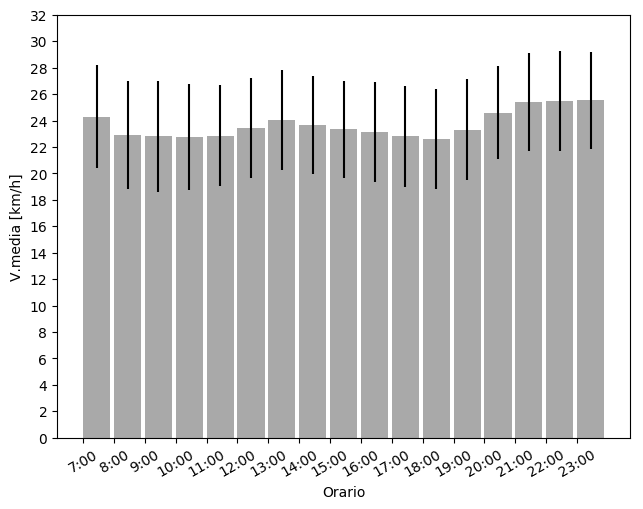
\includegraphics[scale=1.0]{vmedia_oraria_auto}
	\caption{Velocità media in auto [km/h], di ora in ora}
	\label{image:1}
\end{figure}

Una delle prime analisi effettuate per ogni mezzo è stata quella di calcolare la velocità media per ogni tragitto effettuato, con l'obbiettivo di osservare eventuali variazioni di ora in ora. Come riportato visualmente nella figura \ref{image:1}, i tragitti in macchina hanno subito una notevole variazione di velocità media nell'arco 8:00-11:00 e in quello delle 17:00-19:00. Tali risultati sono in linea con quelli dello studio di TomTomIndex\cite{tomtomindexmilan} effettuato sulla città di Milano nel 2019, che evidenzia le ore 9:00 e 18:00, anche dette \textit{rush hours}, come picchi di congestione stradale dal lunedì al venerdì, con un livello di congestione rispettivamente del 70\% e del 60\%. Risultano in linea con lo studio anche le ore precedenti e successive agli orari individuati come picchi.

\subsubsection{Velocità media lunedì-venerdì e sabato-domenica}

\begin{figure}[!h]
	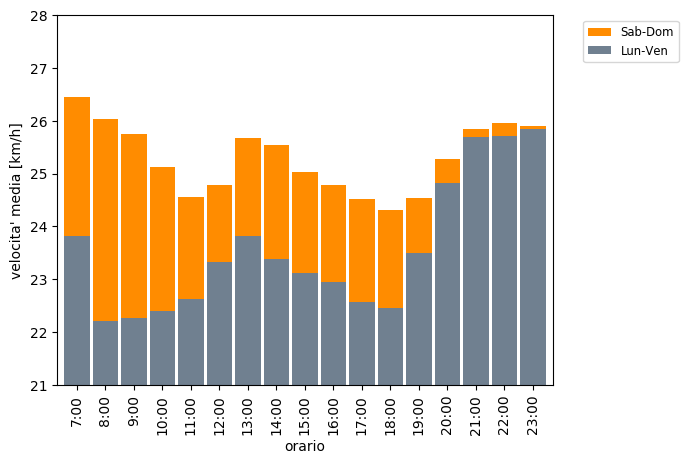
\includegraphics[scale=1.0]{vmedia_oraria_auto_weekend}
	\caption{Velocità media in auto [km/h], di ora in ora}
	\label{image:2}
\end{figure}

La figura \ref{image:2} mostra il risultato di una ripartizione dei dati effettuata sulla base del giorno della settimana, in particolare sono stati divisi i tragitti effettuati dal lunedì al venerdì da quelli del sabato e domenica di ogni settimana. Si può notare una notevole differenza di velocità media indistintamente dall'orario di circa 2 km/h. La variazione nel sabato-domenica risulta meno evidente di quella del lunedì-venerdì, con le variazioni, ovvero i picchi di rallentamento, che si spostanto nelle fasce orarie 10:00-12:00 e 16:00-19:00. Anche questi dati risultano in linea con quelli dello studio di TomTomIndex\cite{tomtomindexmilan}, che vede un minor livello di congestione nel weekend con dei picchi nelle ore 10:00 e 18:00.

\subsubsection{Velocità media settimana dopo settimana da fine lockdown}

\begin{figure}[!h]
	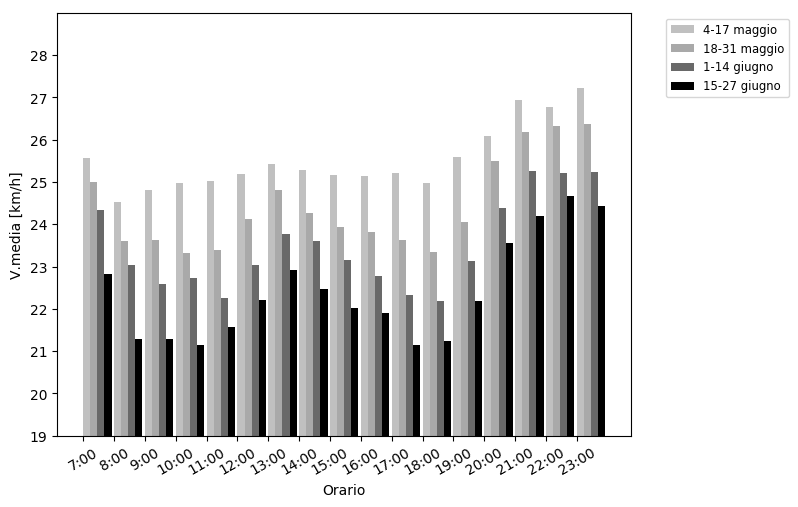
\includegraphics[scale=1.0]{vmedia_oraria_auto_weeks}
	\caption{Velocità media in auto [km/h], di ora in ora}
	\label{image:3}
\end{figure}

La figura \ref{image:3} mostra il risultato di una ripartizione dei dati effettuata in base alla settimana, in particolare sono stati partizionati a gruppi di 2 settimane consecutive i tragitti effettuati a partire dal 4 maggio 2020, primo giorno dell'allentamento delle restrizioni imposte dal governo italiano per l'emergenza covid\cite{dpcm26aprile}. Nel grafico risulta evidente una degradazione della velocità media generale e lineare rispetto al passare delle settimane. Si nota inoltre che le curve corrispondenti alle settimane successive al 17 maggio, ovvero dopo le prime 2 settimane, presentino dei flessi sempre più accentuati in prossimità delle \textit{rush hours} evidenziate dal grafico \ref{image:1}.

\subsection{Enjoy}

\subsubsection{Velocità media di ora in ora}

\begin{figure}[H]
	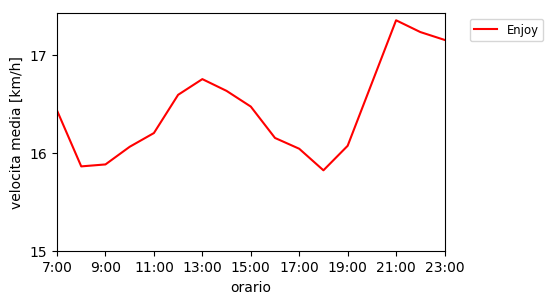
\includegraphics[scale=1.0]{vmedia_oraria_enjoy}
	\caption{Velocità media usando Enjoy [km/h], di ora in ora}
	\label{image:4}
\end{figure}

Siccome le stime di percorrenza col servizio Enjoy sono basate sul servizio di Waze, in particolare il tragitto dalla posizione dell'auto alla destinazione del tragitto, non si riscontrano particolari differenze riguardo i flessi nell'andamento della velocità media di ora in ora osservati nella figura \ref{image:1} per l'auto. La curva però risulta traslata orizzontalmente verso il basso per via del tragitto a piedi necessario per raggiungere un'auto libera che va a influire nel calcolo. Questa traslazione, secondo la figura \ref{image:4}, risulta di circa 5 km/h indipendentemente dall'ora del giorno. Di conseguenza sono state analizzati i dati riguardanti il tragitto a piedi.

\subsubsection{Auto libere e tempo medio per raggiungerle}

\begin{figure}[H]
	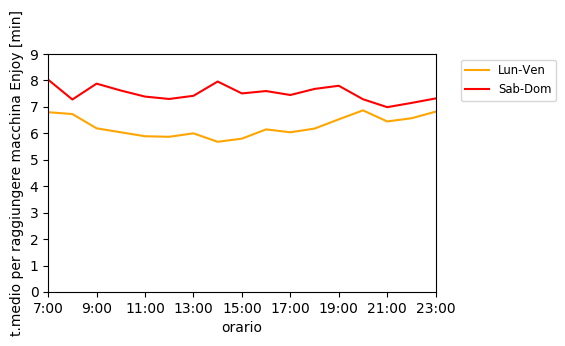
\includegraphics[scale=1.0]{tmedio_raggiungimento_auto_enjoy}
	\caption{Tempo medio per raggiungere auto libera [min], di ora in ora}
	\label{image:5}
\end{figure}

\begin{table}[H]
	\centering
	\begin{tabular}{ | l r | }
		\hline
		& \textbf{ragg. auto} \\
		\textbf{media}   &  6.6 \\
		\textbf{mediana} &  6.0 \\
		\textbf{std}     &  4.6 \\
		\textbf{min}     &  0.0 \\ 
		\textbf{max}     & 43.0 \\
		\hline
	\end{tabular}
	\caption{Statistiche tempo medio per raggiungere auto libera [min]}
	\label{table:4}
\end{table}

Dai calcoli è risultato che il tempo medio impiegato a raggiungere a piedi un'auto del servizio di car sharing Enjoy oscilla intorno ai 6 minuti e mezzo. Anche per questa analisi i dati sono stati partizionati per i giorni da lunedì a venerdì e per sabato e domenica. Il grafico \ref{image:5} mostra una lieve differenza nel tempo medio di circa 1 minuto a favore del primo gruppo, comunemente associato ai giorni lavorativi. A differenza della curva del fine settimana che risulta mediamente stabile, la curva dei giorni lavorativi subisce un calo nel tempo medio nelle ore del primo pomeriggio.

\begin{figure}[H]
	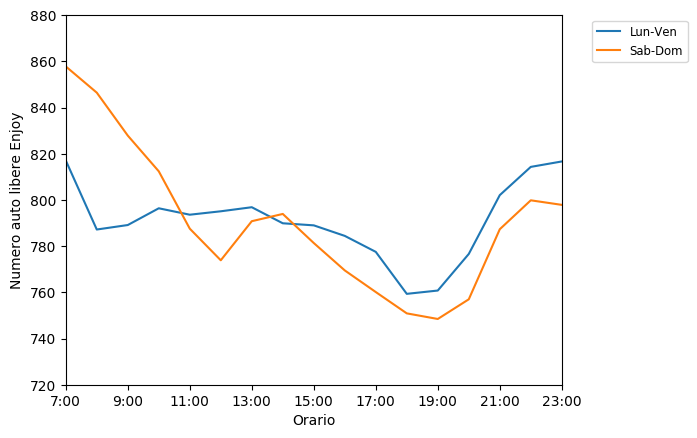
\includegraphics[scale=1.0]{variazione_auto_libere_enjoy_weekend}
	\caption{Numero di auto libere Enjoy lungo l'arco della giornata}
	\label{image:6}
\end{figure}

Per contestualizzare il tempo medio per raggiungere un'auto Enjoy è stato usato il dato sul numero delle macchine libere salvato per ogni query ai servizi. Il massimo numero di auto libere in circolazione è stato di 870. Nel grafico \ref{image:6} viene mostrata in media la variazione di questo conteggio lungo l'arco della giornata, ripartito per lunedì-venerdì e sabato-domenica. Si può notare come il picco di utilizzo del servizio, denotato da un calo delle auto libere a disposizione, inizia verso le 15:00 e finisce verso le 21:00 indipendentemente dal giorno. L'unica differenza tra i due gruppi si può notare nelle ore del mattino, che vede meno auto libere durante la settimana.

\todo{MM: devo inserire il grafico bruttino da vedere?}

Come è stato fatto con la velocità media per l'auto di proprietà, è stato calcolato il tempo medio per raggiungere un'auto libera Enjoy di settimana in settimana dalla fine del lockdown. Il risultato ottenuto è stato controintuitivo, mostrando come, col passare del tempo, il tempo medio per raggiungere un'auto libera diminuiva. Risulta controintuitivo infatti se si pensa al risultato ottenuto con la velocità media in auto, che ha visto una degradazione delle performance col ritorno alla normalità per quanto riguarda la mobilità. Analogamente si è pensato che il numero di utenti del servizio car sharing sarebbe aumentato col ritorno alla normalità e che quindi il tempo medio per raggiungere un auto sarebbe aumentato col diminuire delle auto libere in circolazione. Per investigare a fondo questo risultato è stato calcolato il numero di auto libere di settimana in settimana.

\begin{figure}[H]
	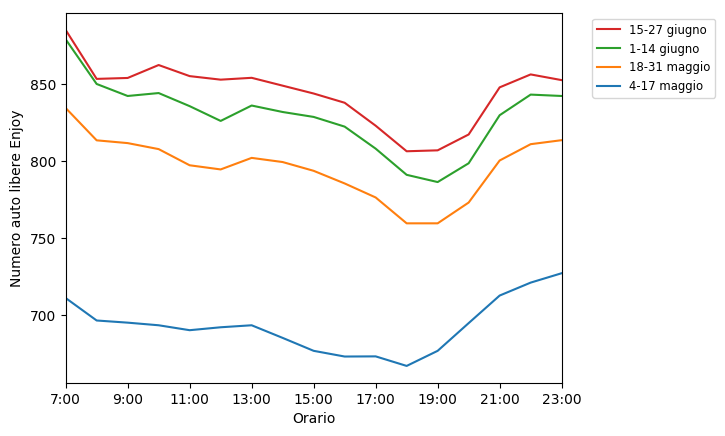
\includegraphics[scale=1.0]{variazione_auto_libere_enjoy_weeks}
	\caption{Numero di auto libere Enjoy lungo settimana dopo settimana}
	\label{image:7}
\end{figure}

Il grafico \ref{image:7} mostra chiaramente come il numero delle auto libere a disposizione sia aumentato con la fine del lockdown. Si può notare infatti come siano state immesse circa 150 nuove auto nell'arco di un mese e altre 50 nel mese successivo. Questo dato di fatto sembra risolvere il risultato controintuitivo ottenuto nell'analisi precedente.


\subsection{ATM, Bici e a piedi}

\subsubsection{Velocità media di ora in ora}

\begin{figure}[H]
	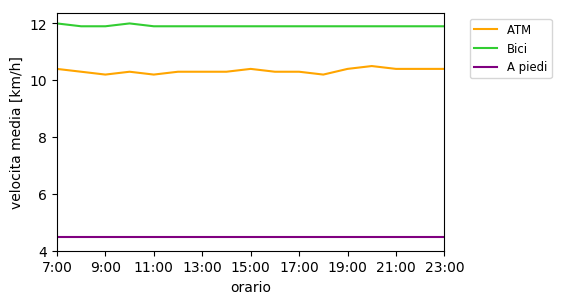
\includegraphics[scale=1.0]{vmedia_oraria_atm_bike_foot}
	\caption{Variazione velocità media di ora in ora}
	\label{image:8}
\end{figure}

Analizzando le stime di percorrenza riguardo i mezzi pubblici, la bicicletta e i percorsi a piedi, non si è verificata alcuna variazione significativa lungo l'arco della giornata, tradotto graficamente come nella figura \ref{image:8} in una retta parallela all'asse x per ognuno dei mezzi considerati. Il risultato ottenuto per la bicicletta e il percorso a piedi è stato ipotizzato, visto che tali mezzi non subiscono gli effetti del traffico nella stessa misura in cui li subiscono le auto e le moto. E' stata analizzata ulteriormente la performance dei mezzi pubblici, che vede una deviazione standard alta ma una performance pressochè costante a qualsiasi ora.

\begin{figure}[H]
	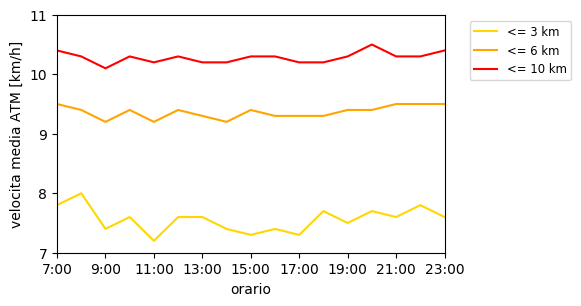
\includegraphics[scale=1.0]{vmedia_oraria_atm_distance}
	\caption{Variazione velocità media con ATM di ora in ora sulla distanza}
	\label{image:9}
\end{figure}

Il grafico \ref{image:9} mostra lo stesso risultato a livello di variazione per qualsiasi lunghezza della tratta. Quel che varia è la velocità media, che vede una differenza di velocità tra le tratte brevi e lunghe.










